
%
% This is the LaTeX source for the instructions to authors using
% the LaTeX document class 'llncs.cls' for contributions to
% the Lecture Notes in Computer Sciences series.
% http://www.springer.com/lncs       Springer Heidelberg 2006/05/04
%
% It may be used as a template for your own input - copy it
% to a new file with a new name and use it as the basis
% for your article.
%
% NB: the document class 'llncs' has its own and detailed documentation, see
% ftp://ftp.springer.de/data/pubftp/pub/tex/latex/llncs/latex2e/llncsdoc.pdf
%
%%%%%%%%%%%%%%%%%%%%%%%%%%%%%%%%%%%%%%%%%%%%%%%%%%%%%%%%%%%%%%%%%%%


\documentclass[runningheads,a4paper]{llncs2e/llncs}

\usepackage{amssymb}
\setcounter{tocdepth}{3}
\usepackage{graphicx}
\usepackage{amsmath}

\usepackage{url}
\newcommand{\keywords}[1]{\par\addvspace\baselineskip
\noindent\keywordname\enspace\ignorespaces#1}

\usepackage{xspace}
%\newcommand{\ie}{\textit{i.e.,}\xspace}
%\newcommand{\eg}{\textit{e.g.,}\xspace}
%\newcommand{\vs}{\textit{v.s.}\xspace}

%

%\mainmatter  % start of an individual contribution

\usepackage{wrapfig}

\sloppy

%%% FORMAT DOCUMENT

\def\textfraction{0}
\def\floatpagefraction{1}
\def\topnumber{3}
\def\bottomnumber{3}
\def\totalnumber{3}
\def\topfraction{1}
\def\bottomfraction{1}

\usepackage[colorlinks]{hyperref}
%\usepackage[inner=2cm,outer=2cm,bottom=2cm,top=3cm]{geometry}
\usepackage{wrapfig}
\usepackage{subfigure}
\usepackage{xspace}
%%%%%%%%%%%%%%%%%%%%%%%%%%%%%%%%%%%%%%%%%
% Acronym of the proposal
\newcommand{\proposal}{DISCUTE\xspace}
%%%%%%%%%%%%%%%%%%%%%%%%%%%%%%%%%%%%%%%%%
%% TODO macros
\usepackage[textwidth=17mm]{todonotes}
  \newcommand{\customtodo}[4]{
        \todo[color=#2,inline,size=\small]{
                \ifx&#3&
                        \textbf{#1} #4
                \else
                        \textbf{#1$\Rightarrow$#3} #4
                \fi
        }
  }
\usepackage{ifthen}
\newboolean{WIP}
\gdef\ifwip{\ifthenelse{\boolean{WIP}}}
%\setboolean{WIP}{false}%
\setboolean{WIP}{true}%
\ifwip{
  \newcommand{\AL}[2][]{\customtodo{AL}{green!50}{#1}{#2}}
  \newcommand{\MS}[2][]{\customtodo{MS}{red!20}{#1}{#2}}
  \newcommand{\JP}[2][]{\customtodo{JP}{blue!20}{#1}{#2}}
  \newcommand{\FQ}[2][]{\customtodo{FQ}{brown!20}{#1}{#2}}
}{ % else if WIP = false
  \newcommand{\AL}[2][]{}
  \newcommand{\MS}[2][]{}
  \newcommand{\JP}[2][]{}
  \newcommand{\FQ}[2][]{}
}
%% End of todo macros
%%%%%%%%%%%%%%%%%%%%%%%%%%%%%%%%%%%%%%%%%
%% Italic abreviations, ...
\newcommand{\ie}[0]{{\em i.e.},\xspace}
\newcommand{\vs}[0]{{\em vs.}\xspace}
\newcommand{\eg}[0]{{\em e.g.},\xspace}
\newcommand{\etal}[0]{{\em et al.}\xspace}
\newcommand{\wrt}[0]{{\em w.r.t.}\xspace}
\newcommand{\aka}[0]{{\em a.k.a.}\xspace}
%%%%%%%%%%%%%%%%%%%%%%%%%%%%%%%%%%%%%%%%%

\begin{document}
% first the title is needed
\title{VMPlaceS – A Generic Tool to Investigate and Compare VM Placement Algorithms}
% the name(s) of the author(s) follow(s) next
%
% NB: Chinese authors should write their first names(s) in front of
% their surnames. This ensures that the names appear correctly in
% the running heads and the author index.
%
\author{Adrien Lebre\inst{1}, Jonathan Pastor\inst{1}, Mario S\"udholt{1}}
%
\authorrunning{A. Lebre, J. Pastor \and M. S\"udholt}
% (feature abused for this document to repeat the title also on left hand pages)

% the affiliations are given next; don't give your e-mail address unless you
% accept that it will be published
\institute{ASCOLA Research Group,
Mines Nantes / Inria / LINA, Nantes, France\\
\email{firstname.lastname@inria.fr}
 }

\maketitle

\begin{abstract}
The use of computing resources provided by cloud companies has become very common. Cloud providers leverage on big datacenters containing tens of thousands of servers. Designing efficient software that can work at this scale is very complex: fault tolerance, network overhead and synchronization can have a significant cost.
\\
A possible solution to minimize these costs is to consider locality properties: servers collaborate first with close servers from the same geographical site. As a result, collaboration between servers can take into account infrastructure parameters such as bandwidth and response time and can be organized in a totally decentralized manner.
\\
This paper shows the case of a large scale virtual machine scheduling algorithm, DVMS, that have been adapted to take advantage of locality properties by using a vivaldi based network overlay. Results of experiments conducted on the grid5000 tesbed, comparing the chord based versus the vivaldi based algorithm, will be presented in the last section.

\keywords{Cloud computing, locality, peer to peer, network overlay, vivaldi, chord, DVMS, virtual machine scheduling}
\end{abstract}

%% Comment this line for submission
%\listoftodos

\subsection{Discovery Initiative}

\begin{itemize}

	\item Users manipulates virtual environment, which is the "gravity center of the IaaS".

	\item Virtual environment contains virtual machines.

\end{itemize}
%\section{The VM Placement Problem}
\label{sec:vmpp}

A VMPP can be summarized in three-steps (see Figure
\ref{fig:scheduling_steps}): monitoring the resources usages,
computing a new schedule each time is it needed and applying the
resulting reconfiguration plan (\ie performing VM migration and
suspend/resume operations to realize to the new placement solution).
% that are mandatory to solve resource violations while optimizing resource usages).

\begin{figure}[ht]
\vspace*{-.2cm}
\begin{center}
        \subcapcentertrue
        \subfigure[Scheduling steps]{
        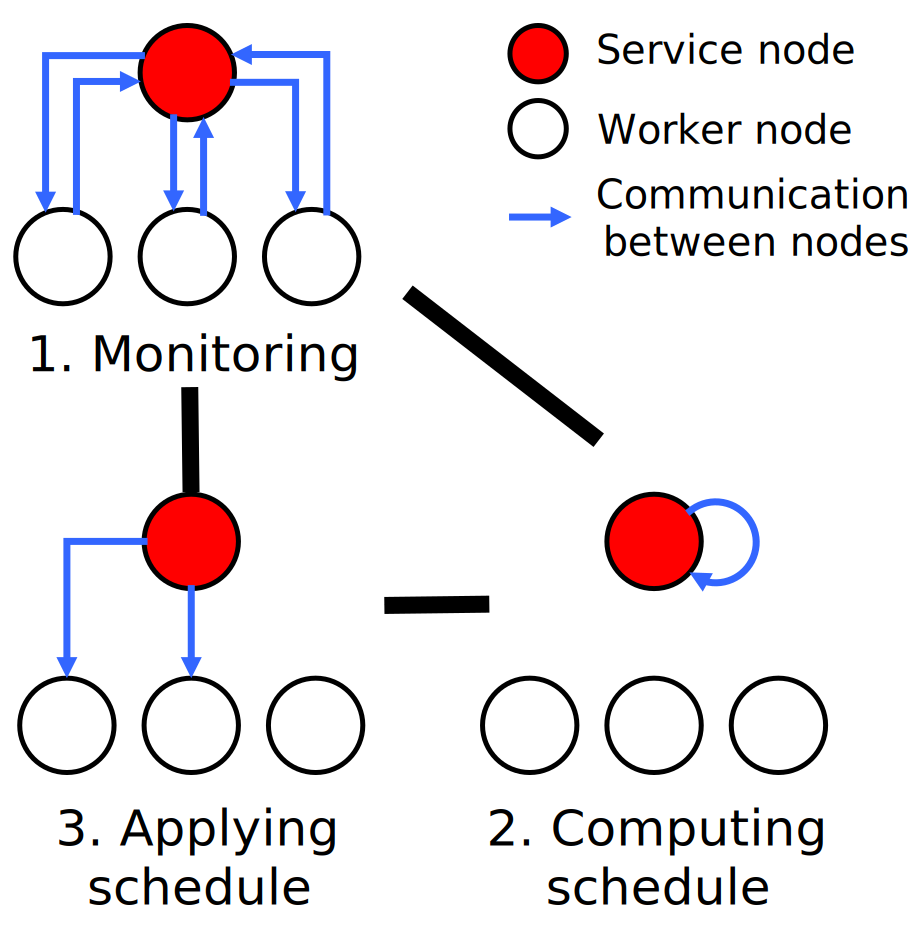
\includegraphics[width=.45\linewidth]{figures/scheduling_steps.pdf}
        \label{fig:scheduling_steps}}
        \subfigure[Workload fluctuations during scheduling]{
        \includegraphics[width=.45\linewidth]{figures/workload_fluctuations2.pdf}
        \label{fig:workload_fluctuations}}
\vspace*{-.2cm}
\caption{VM scheduling Phases}
\end{center}
\label{fig:scheduling}
\vspace*{-.2cm}
\end{figure}
%

VMPP solutions stand and fall with their scalability, reliability and
reactivity of properties, because they have to maintain a placement
that satisfies the requirements of all VMs while optimizing the usage
of CC resources. For instance, a naive implementation of a
master/worker approach as described in
Figure~\ref{fig:scheduling_steps} would prevent workload fluctuations
to be taken into account during the computation and the application of
a schedule, potentially leading to artificial violations (\ie resource
violations that are caused by the VMPP mechanism). In other words, the
longer each phase,
% the longer the reconfiguration process,
the higher the risk that the schedule may be outdated when it is
computed or eventually applied, cf.\ the different loads during the
three phases in Figure \ref{fig:workload_fluctuations}. Similarly,
servers and network crashes can impede the detection and resolution of
resource violations if the master node crashes or if a group of VMs is
temporarily isolated from the master node.

VMPP solutions can only be reasonably evaluated if their behavior in
the presence of such adverse events can be analyzed. Providing a
framework that facilitates such studies and increases their
reproducibility is the main objective of \vmps.



\vspace*{-.05cm}
\section{Simgrid, a Generic Toolkit To Build Simulators}
\label{sec:sg}
%\vspace*{-.05cm}
%\AL[AL]{0.5page}

% Developed for more than a decade,
% and used in a large number of studies described in mor than
% 100~publications,
\sg is a toolkit for the simulation of potentially complex algorithms
executed on large-scale distributed
systems~\cite{casanova:hal-01017319}.
%
To perform simulations, users develop a \emph{program}, and define a
\emph{platform} and a \emph{deployment} files. The \emph{program}
typically leverages \sg's MSG API that allows end users to create
and execute \sg abstractions such as processes, tasks, VMs and network
communications. The \emph{platform} file provides the physical
description of all resources that are the object of the simulation.
% composing the environment and on which aforementioned computations
% and network interactions will be performed in the \sg world.  (host,
% CPU capacity, network topology and link capacities, etc.)
The \emph{deployment} file is used to launch the different \sg
processes of the program on the simulated nodes.
% (at least the mapping between one process and one host is mandatory
% to start the simulation)
Finally, the simulation is orchestrated by the \sg engine that
internally relies on a constraint solver to assign the CPU/network
resources during the entire
simulation.% (for a complete overview see ~\cite{casanova:hal-01017319}).


We chose to base \vmps on \sg
since (i) the latter's relevance in terms of performance and validity
has already been demonstrated~\cite{simgridpub} and (ii) because it
has been recently extended to integrate VM abstractions and a live
migration model \cite{Hirofuchi:2013:ALM:2568486.2568524}. In addition
to enabling researchers to control VMs in the same manner as in the
real world (\eg create/destroy VMs; start/shutdown, suspend/resume and
migrate them), the model implementing the precopy migration algorithm
of Qemu/KVM is the only one that successfully simulates the live
migration behavior by taking into account the competition arising in
the presence of resource sharing as well as the memory refreshing rate
of the VM, thus determining correctly the live migration time as well
as the resulting network traffic. These two capabilities were
mandatory to build \vmps.%our VM placement simulator toolkit.



%%% Local Variables:
%%% mode: latex
%%% TeX-master: "main"
%%% End:

\section{VM Placement Simulator}
\label{sec:injector}

The aim of \vmps is twofold:~(i) to relieve researchers of the burden of
dealing with VM creations and workload fluctuations when they evaluate
new VM placement algorithms and (ii) to offer the possibility to
compare them.
%
% The purpose of \vmps is to deliver a generic tool to evaluate new VM
% placement algorithms and offer the possibility to compare
% them. Concretely, it supports the management of VM creations and
% workload fluctuations.
% % as well as node apparitions/removals.
%  Researchers can
% thus focus on the implementation of new placement algorithms and
% evaluate how they behave in the presence of changes that occur during
% the simulation.
%
% In the following we give an overview of \vmps and describe its
% general functioning.

\subsubsection{Overview.}
\label{sec:overview}

\vmps has been implemented in Java by leveraging the \sg MSG API.
Although Java has an impact on the efficiency
of \sg, we believe its use is acceptable because Java offers important
benefits to researchers for the implementation of advanced scheduling
strategies, notably concerning the ease of implementation of new
strategies. As examples, we implemented the Snooze proposal in Java
and the DVMS proposal using Scala and Java.

\begin{wrapfigure}{r}{.48\linewidth}
\centering
\vspace*{-.6cm}
\includegraphics[width=.99\linewidth]{figures/VMPlaceS-workflow.pdf}
\vspace*{-.5cm}
\caption{\vmps's Workflow}
\flushleft \scriptsize{Gray parts correspond to the generic code while the white one
  must be provided by end-users. %The current version is released with
%  three different schedulers (centralized/hierarchical and
%  distributed).
}
\vspace*{-.8cm}
\label{fig:workflow}
\end{wrapfigure}
%
% From a high-level view,
\vmps performs a simulation in three phases, see
Fig.~\ref{fig:workflow}: (i) initialization, (ii) injection and (iii)
trace analysis.  The initialization phase corresponds to the creation
of the environment, the VMs and the generation of an event queue.
%
The simulation is performed by at least two \sg processes, one
executing the \emph{injector}, the generic part of the framework which
is in charge of injecting the events during the execution of the
simulation, and a second one executing the to-be-simulated
\emph{scheduling algorithm}.
%During the simulation the scheduling
%strategy is evaluated by injecting scheduling-relevant events.
%\AL[MS]{This sentence above is not accurate enough I? previously it
 % was : The
%\emph{injector} constitutes the generic part of the framework. It
%njects scheduling-relevant events during the execution of
%simulations. We should reformulate}
%Currently, the supported events are VM CPU load changes.
% node apparitions/removals that we use to simulate node crashes.
%
The latter analyzes the collected traces in order to gather the
results of the simulation, notably by means of the generation of
figures representing, \eg resource usage statistics.

Researchers develop their scheduling algorithm using the \sg
MSG API and a more abstract interface that is provided by \vmps
and consists of the classes \texttt{XHost}, \texttt{XVM} and
\texttt{SimulatorManager}. The two former classes respectively
extend \sg's \texttt{Host} and \texttt{VM} abstractions while the
latter controls the interactions between the different components of
the simulator.  Through these three classes users can
inspect, at any time, the current state of the infrastructure (\ie the
load of a host/VM, the number of VMs hosted on the whole
infrastructure or on a particular host, check whether a host is
overloaded, etc.).
%We have used \vmps in order to analyze three
%scheduling mechanisms, cf.\ Sec.~\ref{sec:vm-schedulers}, that
%represent three different software architecture models: centralized,
%hierarchical and fully-distributed models for VM placement.
%% TODO
%\MS{The
%  following point is too low-level and should not come here} Although
%we do not discuss that point due to space constraints, we emphasize
%that these three mechanisms enable us to deliver concrete examples of
%how the deployment file of \sg is automatically generated by leveraging
%a generic python script.  \AL{We should highlight that point in the
%  README.org}


%\begin{itemize}
%\item Entropy \cite{Hermenier:2009:ECM:1508293.1508300}, a centralized approach using a constraint programming approach to solve the placement/reconfiguration VM problem;
% \item Snooze \cite{feller:ccgrid12}, a hierarchical approach where
%   each manager of a group invokes Entropy to solve the
%  placement/reconfiguration VM problem. It is noteworthy that in
%   \cite{feller:ccgrid12}, Snooze is using a specific heuristic to solve the placement/reconfiguration VM problem. As the sake of simplicity, we have simply reused the entropy scheduling code.
%\item  DVMS \cite{quesnel:cpe2012}, a distributed approach that dynamically partitions the system and invokes Entropy on each partition.
% \end{itemize}

%\subsection{Initialization Phase}

\subsubsection{Initialization Phase.}

\vmps first creates $n$ VMs and assigns them in a round-robin manner
to the first $p$ hosts defined in the platform file.  The default
platform file corresponds to a cluster of $h+s$ hosts, where $h$
corresponds to the number of hosting nodes and $s$ to the number of
services nodes. The values $n$, $h$ and $s$ constitute input
parameters of the simulations (specified in a Java property file).
%% TODO
% \AL[AL]{Update the size of the cluster autonomically by
%  leveraging p + s}
These hosts are organized in form of topologies, a cluster topology
being the most common one. It is possible, however, to define more
complex platforms to simulate, for instance, federated data center scenarios.
%Note that $s$ can be equals to 0 if the
%scheduling strategy is directly executed on the hosting nodes.

Each VM is created based on one of the predefined VM classes. A VM
class corresponds to a template specifying the VM attributes and its
memory footprint. It is
% described as
% \texttt{nb\_cpu:ramsize:net\_bw:mig\_speed:mem\_speed}
defined in terms of five parameters: the number of cores
\texttt{nb\_cpus}, the size of the memory \texttt{ramsize}, the
network bandwidth \texttt{net\_bw}, the maximum bandwidth available
% migrate it
\texttt{mig\_speed} and the maximum memory update speed
\texttt{mem\_speed} available when the VM is consuming 100\% of its
CPU resources.  Available classes are defined in a text file that is
modifyable by users.  As pointed out in Section \ref{sec:sg}, the
memory update speed is a critical parameter that governs the migration
time as well as the amount of transferred data.  VM classes provide
means to simulate arbitrary kinds of workload (\eg memory-intensive
ones) % , and thus analyze more realistic CC problems.

%\MS{Follows a low-level mechanism!}
% TODO not addressed yet. This text should appear in the README
%At creation time
%of a VM, a process selects one class (\ie one line) in the file
%randomly. Hence, if a user wants to favor a specific class, he can
%simply repeat the line of the class several times.
%
All VMs start with a CPU consumption of 0 that will evolve during the
simulation depending on the injected load as explained below.
%
Once the creation and the assignment of VMs completed, \vmps spawns at
least two \sg processes, the \emph{injector} and the launcher of the
selected scheduler.  At its start the \emph{injector}
% consists in creating the different event queues and merge them into
creates an event queue that will be consumed during the second phase
of the simulation.  Currently, \vmps supports \emph{CPU
  load change} events (only).
%and
%\emph{node crash} events.
%\todo{Before apparitions/ removals}
% The former consists in changing the load of a VM by creating and
% assigning a new \sg task in the VM while the second aims at
% simulating crashes.
%
% Changing the load of a VM has a direct impact of its memory update
% speed and thus on the time to migrate it between two hosts.
The event queue is generated in order to change the load of each VM
every $t$ seconds on average. $t$ is a random variable that follows an
exponential distribution with rate parameter $\lambda_t$ while the CPU
load of a VM evolves according to a Gaussian distribution defined by a
given mean ($\mu$) as well as a given standard deviation
($\sigma$). $t$, $\mu$ and $\sigma$ are provided as input parameters
of a simulation.
% As the CPU load can fluctuate between 0 and 100\%, \vmps prevents
% the assignment of nonsensical values when the Gaussian distribution
% returns a number smaller than 0 or greater than 100.
% Although this has no impact on the execution of the simulation,
% we emphasize that this can reduce/increase the effective mean of the
% VM load, especially when $\sigma$ is high.  Hence, it is important for
% users to specify appropriate values.
%% TODO
%\AL[AL]{A binomial law would have solved this issue: too late too bad :(}
%Although this can have an impact on the
%effective mean, especially when $\sigma$ is high, we believe it was
%non appropriated to request it is easier for end-users to specify $\mu$ and
%$\sigma$ parameters than
Furthermore, each random process used in \vmps is initialized with a
seed that is defined in a configuration file. This way, we can ensure
that different simulations are reproducible and may be used to
establish fair comparisons.

%The \emph{node crash} event queue is generated in order to turn off a
%node every $f$ seconds on average for a duration of $d$ seconds.
%Similarly to the $t$ value above, $f$ follows an exponential
%distribution with rate $\lambda_f$. $f$ and $d$ are also provided as
%input parameters of a simulation.

Finally, we highlight that adding new events can be done by simply
defining new event Java classes implementing the
\texttt{InjectorEvent} interface and by adding the code in charge of
generating the corresponding events that are then handled
% the associated queue. Such a
% new queue will be merged into the global one and its events will then be
% consumed
similarly to the \emph{CPU Load}
ones.% during the \emph{injector phase}.
As an example, the next release of \vmps will integrate \emph{node
  apparition/removal events} that will be used to simulate crashes.

\subsubsection{Injector Phase.}

Once the VMs and the global event queue are ready, the evaluation of
the scheduling mechanism can start. First, the injector process
iteratively consumes the different events.  Changing the load of a VM
corresponds to the creation and the assignment of a new \sg task in
the VM. This new task has a direct impact on the time that will be
needed to migrate the VM as it increases or decreases the current CPU
load and thus % the percentage of
its memory update speed.
% \MS[AL]{Is the above paragraph clear enough?}
% that is indicated by the \texttt{mem\_speed}
%% parameter given in the class description.
%When a node is turning off, the VMs that were running on that node are
%temporarily discarded, \ie they are hidden and cannot be accessed
%until the node comes back to life. This way, the scheduler cannot
%handle them.
 %\AL[AL, MS, JP]{This is ugly but unfortunately the true,
 % it will be better to reassign those VMs on other nodes, but which
 % one?  }
%We leave for future work other approaches that can better
%match realistic scenarios such as turning off the VMs and
%reprovisioning them on other nodes.
%

Based on the scheduler decisions, VMs will be suspended/resumed
or relocated on the available hosts.
% to meet scheduling objectives.  and SLA guarantees.
Users must implement the algorithm in charge of solving the VMPP but
also the code in charge of applying reconfiguration plans using
methods from the \texttt{SimulatorManager} class. This step is
essential as the reconfiguration cost is a key element of dynamic
placement systems.

% \MS[AL]{maybe it is better to prevent the access to Xhost
%   and XVM methods that can change the Simulator States. Hence, we
%   should enforce the access only through the SimulatorManager class?
%   What do you think? Yes, would be cleaner. Can we just present the
%   interface as such? Or not talk about the direct possibility?}
It is noteworthy that \vmps invokes the execution of each scheduling
solver, as a real implementation would do, to get the effective
reconfiguration plan.  That is, the computation time that is observed
is not simulated but corresponds to the effective one, only the
workload inside the VMs and the reconfiguration operations (\ie
suspend/resume and migrate) are simulated in \sg.
% It is hence mandatory to propagate the effective computation time
% into the \sg engine.%
% The following is IMO a technical detail by invoking a \texttt{wait}
% call of the MSG interface.

\subsubsection{Trace Analysis.}
\label{subsec:traces-analysis}

The last step of \vmps consists in analyzing the information that has
been collected during the simulation.
% in order to understand and compare the behavior of the different
% algorithms.
This analysis is done in two steps. First, \vmps records several
metrics related to the platform
utilization % throughout the simulation
using an extended version of \sg's TRACE
module\footnote{\url{http://simgrid.gforge.inria.fr/simgrid/3.12/doc/tracing.html}}.
This way, visualization tools that have been developed by the \sg
community, such as PajeNG~\cite{pageng:www}, may be used with
\vmps. Furthermore, our extension enables the creation of a JSON trace
file, which is used to represent resource usage by figures generated
using the R statistical environment~\cite{R:Bloomfield:2014}.

By default, \vmps records the load of the VMs and hosts, the
start and the duration of each violation of VM requirements in
the system, the number of migrations, the number of times the
scheduler mechanism has been invoked and the number of times it
succeeds or fails to resolve non-viable configurations.
%
% Although these pieces of information are key elements to understand
% and compare the behavior of the different algorithms, we emphasize
% that
The TRACE API is extensible in that as many variables as necessary can
be created by users of our system, thus allowing researchers to
instrument their own algorithm with specific variables that record
other pieces of information.




%%% Local Variables:
%%% mode: latex
%%% TeX-master: "main"
%%% End:
%

\section{Dynamic VMPP Algorithms}
\label{sec:vm-schedulers}

To illustrate the interest of \vmps, we implemented three dynamic VM
placement mechanisms: a centralized one based on the Entropy
proposal~\cite{Hermenier:2009:ECM:1508293.1508300}, a hierarchical one
based on Snooze~\cite{feller:ccgrid12}, and a fully-distributed one
based on DVMS~\cite{quesnel:cpe2012}.

\MS{We should differentiate more clearly between the complete VMPP
  system and the solver.}

These systems enable  the resolution  of violations in form of
overloaded nodes. A host is overloaded when the VMs try to consume
more than 100\% of the CPU capacity of the host. In such a case, a
resolution algorithm looks for an optimal viable configuration until
it reaches a predefined timeout. In all cases, we chose to use the
latest solver developed as part of the Entropy
framework~\cite{hermenier:cp11} as this resolution algorithm.
% Giving up consolidation optimality in favor of scalability, this
% algorithm provides a ``repair mode'' that enables the correction of VM
% requirement violations. The optimal solution is a new placement that
% satisfies the requirements of all VMs while minimizing the cost of the
% reconfiguration.
Once the timeout has been triggered, the algorithm returns the best
solution among the ones it finds and applies the associated
reconfiguration plan by invoking live migrations in the simulation
world.
%
% Although using the Entropy VMPP solver implies a modification from the
% original Snooze proposal, we highlight that our goal is to
%
% and thus we believe that such a modification is acceptable as it
% does not change the global behavior of Snooze

Simulating these three VMPP systems illustrates the capabilities of
\vmps. Moreover, by conducting such a comparison, we also investigate
the pros and cons of the three architecture models on which these
proposals rely on (\ie centralized, hierarchical and distributed).

In the remainder of this section, we first present an overview of the
three systems, showing, in particular, that the extended abstractions
for hosts (\texttt{XHost}), VMs (\texttt{XVM}) and the functions of
the \sg MSG API enabled us to develop them in a direct and natural
manner. We then present simulation results that, as a first, allow the
three approaches to be compared.

\subsection{Entropy-based Centralized Approach}
\label{subsec:entropy}
The centralized VM placement mechanism consists in one single \sg
process deployed on a service node. This process implements a simple loop that
iteratively checks the viability of the current configuration by
invoking seconds the aforementioned VMPP solver with a predefined
frequency.
% $p$ is defined as an input parameter of the simulation.

% \AL{Should we explain the issue right now or not if we add VMPP section}
% Indeed, during
% the computation and the application of a schedule, the algorithm does
% not enforce QoS properties anymore, and thus cannot react quickly to
% violations. Second, since the manipulation of VMs is costly, the time
% needed to apply a new schedule is particularly important: The longer
% the reconfiguration process is, the higher is the risk that the schedule may
% be outdated, due to the workload fluctuations, when it is eventually
% applied.
% \vmps enables researchers to investigate such concerns in-depth.

% As the Entropy proposal does not provide a specific mechanism for the
% collection of resource usage information but simply uses an external
% tool (namely ganglia), we had two different ways to implement the
% monitoring to process: either by implementing additional asynchronous
% transmissions as a real implementation of the necessary state updates
% would proceed or, in a much more lightweight manner,
We monitor the resource usage through direct accesses
% by the aforementioned process
to the states of the hosts and their respective VMs, while accounting
for communication overheads explicitly
% induced by communication in the ``real'' implementation, for
% instance, can be easily added as part of the lightweight
% simulation. We have implemented this lightweight variant for the
% monitoring
%
% Regarding fault tolerance, similarly to the Entropy proposal, our
% implementation does not provide any failover mechanism.
%
% as mentioned in Section \ref{subsec:traces-analysis},
We also monitor, for each iteration, whether the VMPP solver succeeds
or fails. In case of success, \vmps records the number of migrations
that have been performed, the time it took to apply the
reconfiguration and whether the application of the reconfiguration
plan led to new violations.

\subsection{Snooze-based Hierarchical Approach}
\label{subsec:snooze}
We now present Snooze~\cite{feller:ccgrid12} as a second case study of how
to implement and simulate advanced algorithms.
We present its architecture summarizing its main
characteristics from its original presentation~\cite{feller:ccgrid12} and
additional information  stemming from personal communications of the Snooze
developers and its implementation~\cite{snoozeweb,snoozedev14}.

\subsubsection{Architecture}
\label{sec:snoozeArchi}

Snooze harnesses a hierarchical architecture in order to support load
balancing and fault tolerance, cf.\ Fig.~\ref{fig:snoozearch}.

\begin{figure}[hbp]
  \begin{center}
  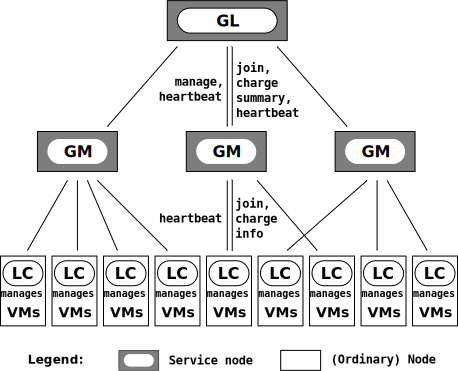
\includegraphics[width=.85\linewidth]{figures/snoozearch.pdf}
  \caption{Overview of Snooze's architecture}
  \label{fig:snoozearch}
\end{center}
\vspace*{-.3cm}
\end{figure}

At the
top of the hierarchy, a \emph{group leader (GL)} centralizes
information about the whole cluster using summary data about
\emph{group managers (GMs)} that constitute the intermediate layer of
the hierarchy. GMs manage a number of \emph{local controllers (LCs)}
that, in turn, manage the VMs assigned to nodes. The GL and the GMs
are deployed on service nodes while the LCs are executed on hosting
node.  During execution, higher-level components periodically send
heartbeats to lower-level ones; monitoring information, \eg about the
system load, is also sent periodically in the opposite direction. In
order to propagate information down the hierarchy, Snooze relies on
hardware support for multicast communication. Finally, a number of
replicated entry points allows clients to contact the GL, \eg in order
to submit new VMs for integration into the system.

\emph{Simulation using \vmps.~} The \texttt{XHOST}, \texttt{XVM} and
\texttt{SimulatorManager} classes have been harnessed to implement the
core architectural abstractions (\ie VM monitoring and manipulations),
the remaining concepts and algorithms of Snooze have been implemented
using Simgrid's primitives and standard Java mechanisms.
%
Communication between Snooze actors is implemented based on Simgrid's
primitives for, mainly asynchronous, event handling.
Hardware\-sup\-ported multicast communication that is used, \eg
to relay heartbeats, is implemented as a dedicated actor that manages
a state representing GL and GM heartbeat groups and relaying heartbeat
events.
%
Finally, our Snooze simulation uses, as its original counterpart, a
multi-threaded implementation (\ie based on multiple SG processes) in
order to optimize reactivity even for large groups of LCs (or GMs)
that have to be managed by one GM (or GL).

\subsubsection{Algorithms}
\label{sec:snoozeAlgs}

Apart from the handling of faults (described below), two types of
algorithms are of major importance for the administration of the
Snooze architecture: the algorithms that enable components to
dynamically enter the system and the algorithms that propagate info
between the components.

A GL is created, if it does not exist, by promotion of a GM that is
selected according to some leader election algorithm. When a GM joins
a cluster, it starts listening on a predefined channel for the
heartbeat of the GL and registers once it has received the
heartbeat. New LCs first also wait for the GL heartbeat, contact the
GL then in order to obtain a GM assignment, and finally register at
the GM assigned to them.

Two kinds of (load) information are passed within the system: the
periodic heartbeat message sent by the GL and the GMs; second,
periodic load information sent from LCs to their respective GMs and
summary load info sent by the GMs to the GL.

\subsubsection{Fault tolerance}

GLs, GMs and LCs may fail during the system execution. System
components identify that a node on the corresponding higher-level node
has failed (the GL in case of a GM, a GM in the case of an LC) in an
asynchronous fashion through the lack of heartbeat messages.

In the case of a GL failure, one of the GMs becomes the new GL, stops
its GM activities and prevents the LCs it manages so that they can
start rejoining the system. If a GM fails, the GL and the LCs it has
managed will become aware of it based on the lack of heartbeats,
update its data structures and, for the LCs, rejoin the system. If an
LC fails, its GM will finally learn of it due to the missing heartbeat
and charge information of the LC. The GM will then remove the LC from
its data structures.


% \subsubsection{Variants}
% \label{sec:snoozeVariants}

% Our simulation framework facilitates the simulation of variants of
% placement algorithms. In the following, we present three non-trivial
% variants that we have implemented and explored: a variant of the
% assignment algorithm of LCs to GMs, periodic vs.\ reactive scheduling,
% and a variant of the algorithms of how GMs and LCs join the system.


% \paragraph{Assignment of LCs to GMs}

% LCs are assigned to GMs by the GL as part of the LC join protocol. In
% Snooze's native implementation LCs are assigned in a round-robin
% fashion to the known GMs. If GMs join (and leave) the system at the
% same time as LCs, a round-robin strategy at join time, however, does
% not ensure an even distribution. This may happen, for instance at
% startup time of the system, when new GMs and LCs enter the system, or
% in case of failures, which trigger GM and LC joins. In order to
% evaluate the imbalance resulting from a round-robin strategy (as well
% as others) we have implemented the LC assignment protocol in a modular
% fashion and applied it in diverse highly-dynamic settings in which GMs
% and LCs enter the system at the same time. Furthermore, we have
% implemented a best-fit strategy that assigns LCs to GMs with minimal
% load or to GMs with the smallest number of assigned LCs (if several
% GMs with minimal load exist). The best-fit strategy can significantly
% improve the scheduling characteristics of hierarchical placement
% algorithms as shown by the experimental data presented in
% Sec.~\ref{sec:snoozeVariantsEval}. Furthermore, it should always be
% at least as good as the round-robin strategy (the corresponding proof
% is left to future work).


% \paragraph{Periodic vs.\ reactive scheduling}

% Snooze~\cite{feller:ccgrid12} schedules VMs in a periodic fashion:
% after a fixed time period a GM calls the scheduler in order to resolve
% resource conflicts among the LCs it manages. The information whether a
% resource conflict has to be handled is taken based on the summary
% information that is periodically sent by the LCs to the GM.

% We have provided an alternative, reactive, strategy to scheduling: as
% soon as they occur, LCs avert their GMs of resource conflicts; the GMs
% then initiate scheduling. Implementing this reactive scheme can be
% done using our framework in two manners: either by implementing
% additional asynchronous transmissions as a real implementation of the
% necessary state updates would proceed or, in a much more lightweight
% manner, through direct accesses by the GMs to the states of their
% respective LCs. While the latter does not mimic a real implementation
% closely, it can be harnessed to yield a valid simulation: delays
% induced by communication in the ``real'' implementation, for instance,
% can be easily added as part of the lightweight simulation. We have
% implemented this lightweight variant of reactive scheduling.


% \paragraph{Variants of the join algorithms}

% The join algorithms, see Sec.~\ref{sec:snoozeAlgs}, are crucial to the
% correctness of Snooze for two main reasons: (i) they have to be
% efficient because they can easily form a bottleneck if large numbers
% of LCs (GMs) have to be registered at a GM (LC); (ii) they are
% multi-phase protocols whose correctness especially in the presence of
% faults is difficult to ensure.

% In order to investigate the corresponding trade-offs, we have used our
% framework to implement join algorithms that may be interrupted at any
% time, repeat the the on-going phase a number of times before
% reinitiating, if necessary, the entire protocol. Furthermore, the join
% protocol is parameterized, \eg, in the number of threads used to
% handle registration requests.

% Finally, our framework has enabled us to test another aspect of
% Snooze's join algorithm as presented by
% Feller~\etal.~\cite{feller:ccgrid12},
% \MS[MS]{If we succeed to perform the experiment comparing both
%   approach, this paragraph should be highlighted.}
% a strategy we call the GM rejoin
% strategy (GRJ): all GMs should rejoin if a new GM enters the
% system. While GRJ supports a form of load balancing (because all LCs
% are reassigned to the new set of GMs), our simulation has shown that
% this strategy significantly increases the time necessary for
% registering GMs and LCs compared to a simpler strategy that does not
% modify existing GMs in case a new GM enters the system. This handicap
% is particularly pronounced if joins of GMs may be interrupted due to
% faults. Concretely, experiments involving 20 GMs and 200 LCs have
% shown that this strategy often multiplies the time necessary to join
% all 220 components by 10 or more compared to the simple join
% strategy. While the qualitative result that the more complex strategy
% presented in the paper results in a more time-consuming join process
% is not very surprising, the extent of the resulting degradation was
% surprising.



%%% Local Variables:
%%% mode: latex
%%% TeX-master: "main"
%%% End:


\subsection{DVMS-based Distributed Approach}
\label{subsec:dvms}
% TODO Not adressed
%\AL[AL]{Check who write that part, If Flavien did it, then add him as
%  an author}
DVMS~\cite{quesnel:cpe2012} (Distributed Virtual Machine
Scheduler) is a framework that schedules VMs cooperatively and dynamically in
large-scale distributed systems.

\subsubsection{Overview and Definitions}
From a software point of view, the nodes are organized following a ring
topology.

A scheduling procedure is started as soon
as an event occurs on the infrastructure.

Each event is associated with a partition.  A partition is composed of all the
nodes that are reserved for the resolution of a specific event.
%
Partitioning the infrastructure is mandatory to avoid conflicts between several
schedulers that could manipulate the same nodes or VMs when they apply their
reconfiguration plans.

Each partition includes two special nodes, the initiator and the leader.
The initiator of a partition is the node that
initially produced the event associated with this partition.
The leader of a partition is the node that leads the scheduling computations
aiming at solving the event associated with this partition; the leader of
the partition is likely to change during the processing of the event.


\subsubsection{The Problem Solving Procedure}

The problem solving procedure is initiated when a node
N\(_{\textit{i}}\) observes that there is a problem, for instance when its
resources are overused (see Figure~\ref{fig:dvms_pte}); it then generates an
event and reserves itself to process this event (see
Figure~\ref{fig:dvms_pte_1}).  After that, it forwards this event to its
neighbor on the ring, node N\(_{\textit{i+1}}\).

If N\(_{\textit{i+1}}\) is already involved in another partition, it directly
forwards the event to node N\(_{\textit{i+2}}\); otherwise, N\(_{\textit{i+1}}\)
joins the new partition (see Figure~\ref{fig:dvms_pte_2}) and checks that the
event is still valid.  If the event is not valid anymore (for instance because
the virtual machines demands for resources fluctuated), N\(_{\textit{i+1}}\)
cancels the reservations to destroy the partition and thus allow the nodes that
composed it to take part to other problem solving procedures.
%
On the contrary, if the event is still valid, N\(_{\textit{i+1}}\) notifies all
the nodes inside the partition that it is the new leader; in return, it receives
information regarding (i)~the capacities of each node and (ii)~the resources
consumed by the virtual machines hosted on each node.  It then starts a
scheduling computation; if no solution is found, the event is then forwarded to
node N\(_{\textit{i+2}}\).

N\(_{\textit{i+2}}\) repeats the same operations, that is to say: self-reservation
(if it is free, see Figure~\ref{fig:dvms_pte_3}), event validity check, leader
change notification, monitoring of VMs and nodes inside the partition,
scheduling computation.  If N\(_{\textit{i+2}}\) finds a solution, it applies the
corresponding reconfiguration plan that solves the event; it then cancels
reservations to destroy the partition and thus allow the nodes that composed it
to take part to other problem solving procedures.

Note that, if N\(_{\textit{i+2}}\) did not find a solution, the partition would
have grown until a solution was found or the even had traversed the whole ring.
In the latter case, the problem would be considered as unsolvable and the
partition would be destroyed.

The progressing increase in size of the partition aims at adapting it to the
complexity of the problem to solve.
This approach enables to consider as few nodes as possible, thus accelerating
the scheduling computations to solve the event as quickly as possible.

\begin{figure}[h]
\subfigure[]{
\includegraphics[width=3.8cm]{./figures/fig-24.pdf}
\label{fig:dvms_pte_1}}
%
\subfigure[]{
\includegraphics[width=3.8cm]{./figures/fig-25.pdf}
\label{fig:dvms_pte_2}}
%
\subfigure[]{
\includegraphics[width=3.8cm]{./figures/fig-26.pdf}
\label{fig:dvms_pte_3}}
%
\subfigure[Legend]{
\includegraphics[width=3.8cm]{./figures/fig-27.pdf}
\label{fig:dvms_pte_4}}
%
\caption{Processing two events simultaneously\label{fig:dvms_pte}}
\end{figure}


\subsubsection{Fault-tolerance}

The original implementation of DVMS was not fault-tolerant.


\paragraph{Repairing the Ring.}

Making DVMS fault-tolerant implied first to make the ring fault-tolerant.
Previously, if a node \emph{N\(_{\textit{i}}\)} crashed, an event passing through
node \emph{N\(_{\textit{i-1}}\)} could not reach node \emph{N\(_{\textit{i+1}}\)}.

To preserve the integrity of the ring, we used the algorithms
designed for Chord~\cite{stoica:2001:sigcomm01}.
%
The main idea is to let each node know not only its neighbor, but also its
2\(^{\textit{1}}\) successor, its 2\(^{\textit{2}}\) successor, and so on until the
2\(^{\textit{i}}\) successor, \emph{i} being specified by the administrator;
%
when some part of the ring crashes, network communications can still be
performed by passing through a known alive successor.


\paragraph{Destroying a Partition If One of Its Node Fails.}

Having a fault-tolerant ring was not enough; it was also necessary to make the
problem solving procedure fault-tolerant.

Previously, if the leader of a partition crashed, the problem identified by the
initiator would never be solved; moreover, the nodes of this partition would
remain reserved indefinitely and would not be able to take part to other problem
solving procedures.

To avoid these issues, DVMS now relies on a timeout.  Each node involved in a
partition periodically checks whether the state of its partition changed
recently (for instance, a new node joined the partition).
%
If the state does not change anymore, it probably means that the problem solving
procedure is stuck (maybe because the leader crashed).
%
In this case, each node decides to leave the partition and becomes free to take
part to other problem solving procedures.




%%% Local Variables:
%%% mode: latex
%%% TeX-master: "main"
%%% End:

\section{Experiments}
\label{sec:experiments}

%\AL[JP,AL,MS]{2 pages}
% In this section, we, first, analyze the accuracy of \vmps by comparing
% the  results of an Entropy execution through simulations and
% \textit{in-vivo} experiments. This first experiment enables us to
% confirm the expected behavior of \vmps Second, we present and discuss
% our analysis of the three algorithms previously described.
% We show that the performances of the hierarchical approach could
% reached the distributed ones through minor changes.

Two kinds of experiments have been performed to validate the relevance
of \vmps. The objective of the first one was to evaluate the accuracy
of the returned results while the second was a concrete use-case of
\vmps, analyzing the three strategies introduced before.

\subsection{Accuracy Evaluation}
\label{subsec:accuracy}

To validate the accuracy of \vmps, we have implemented a dedicated
version of our
framework\footnote{\url{https://github.com/BeyondTheClouds/G5K-VMPlaceS}}
on top of the Grid'5000 testbed and compared the execution of the
Entropy strategy invoked every 60 seconds over a 3600 seconds period
in both the simulated and the real world.  Regarding the
\textit{in-vivo} conditions, experiments have been performed on top of
the Graphene cluster (Intel Xeon X3440-4 CPU cores, 16 GB memory, a
GbE NIC, Linux 3.2, Qemu 1.5 and SFQ network policy enabled) with 6
VMs per node.  Each VM has been created using one of 8 VM predefined
classes.
The template was 1:1GB:1Gbps:1Gbps:X, where the memory update
speed X was a value between 0 and 80\% of the migration bandwidth
(1Gbps) in steps of 10. Starting from 0\%, the load of each VM varied
according to the exponential and the Gaussian distributions. The
parameters were $\lambda$ = \#VMs/300 and $\mu$= 60, $\sigma$ = 20.
Concretely, the load of each VM varied on average every 5 min in steps
of 10 (with a significant part between 40\% and 80\%). A dedicated
\texttt{memtouch} program~\cite{Hirofuchi:2013:ALM:2568486.2568524}
has been used to stress both the CPU and the memory
accordingly.
Regarding the simulated executions, \vmps has been
configured to reflect the \textit{in-vivo} conditions.
In particular,
we configured the network model of SimGrid
%\begin{figure}[hbt]
\begin{wrapfigure}{r}{.50\linewidth}
\centering
\vspace*{-.75cm}
%\includegraphics[width=0.99\linewidth]{./figures/simu-vivo-32PM-192VM-6020-original.pdf}
% \subcapcentertrue
%\subfigure{
\includegraphics[width=1.1\linewidth]{./figures/accuraci-simu.pdf}
%\label{fig:accu-simu}}
%\subfigure{
\vspace*{-.6cm}\includegraphics[width=1.1\linewidth]{./figures/accuraci-invivo.pdf}
%\label{fig:accu-vivo}}
\vspace*{-.32cm}
\caption{Comparison between simulated (top) and \textit{in-vivo}
  (bottom) Executions}
\vspace*{-.28cm}
\flushleft\scriptsize{The Y-axis represents the duration of each Entropy
  invocation. It is divived into two parts: the time to look for a
  new configuration (the computation phase in red) and the time to
  relocate the VMs (the reconfugration phase in black). Both axis are
  in seconds.
%  perform each reconfiguraton (red parts correspond the computation
%  phase,  (\ie
%  the time where Entropy looks for a new configuration). The black parts correspond to the reconfiguration phase (\ie when
%VM are relocated throughout the cluster.
}
\label{fig:usecase-vivosimu}
\vspace*{-.9cm}
\end{wrapfigure}
%\end{figure}
in order to cope with the network performance of the Graphene servers that were allocated to our
experiment (6 MBytes for the TCP gamma parameter and 0.88 for the
bandwidth corrective simulation factor).
%
Fig.~\ref{fig:usecase-vivosimu} shows the time to perform the two phases of
the Entropy algorithm for each invocation when considering 32~PMs and
192~VMs through simulations (top) and in reality (bottom). Overall, we can see that simulation results successfully
followed the in-vivo ones. During the first hundreds seconds, the cluster did not
experience VM requirement violations because the loads of VM were
still small (\ie Entropy simply validated that the current placement
satisfied all VM requirements). At 540 seconds, Entropy started to
detect non viable configurations and performed reconfigurations.
Diving into details, the difference between the \textit{simulated} and
\textit{in-vivo} reconfiguration time fluctuated between 6\% and 18\%
(median was around 12\%). %during the experiment.
The worst case, \ie 18\%, was reached when
multiple migrations were performed simultaneously on the same
destination node.
 In this case and even if the SFQ network policy was
enabled, we discovered that in the reality the throughput of migration
traffic fluctuated when multiple migration sessions simultaneously
shared the same destination node. We confirmed this point by analyzing
TCP bandwidth sharing through \texttt{iperf} executions. We are
currently investigating with the \sg core-developers how we can
integrate this phenomenon into the live-migration model. However, as a
migration lasts less than 15 seconds in average, we believe that that
the current simulation results are sufficiently accurate to capture
performance trends of placement strategies.


% As an example, we noticed that applying the
% reconfiguration plan was much more time-consuming than computing it. This result that has been correctly reported by the simuations means that VMPP also needs
% to address the way of shorten reconfiguration phases, not only that of
% computing ones.
% % This is rather important as most relocation
% % algorithms try to reduce the computation phase instead of focusing on the
% % reconfiguration one.
% Leveraging \vmps will enable researchers to observe such key points
% without facing with the burden of conducting large scale
% \textit{in-vivo} experiments. We illustrate such an advantage in the
% following section.




%%% Local Variables:
%%% mode: latex
%%% TeX-master: "main"
%%% End:

%\subsection{A First Use-Case:  Comparison of Entropy, Snooze and DVMS}
\subsubsection{Analysis of Entropy, Snooze and DVMS}
\label{subsec:first-usecase}
%\AL{Il faudra parler du nombre de migrations qui est egalement une
%  métrique pertinente. Plusieurs algorithms tentent de reduire cette
%  metrique }
%\AL[AL]{Il faudra mettre des snapshots de PajeNG}
% Evaluation of VMPlaceS on Grid'5000: simulations were running on one server.
In this paragraph, we discuss the results of the simulations we
performed on the Entropy,  Snooze and DVMS strategies.
% Due to space limitations we present a generaly study
% analyzing the violation times as well as the
% duration of the computation and reconfiguration phases. However, we
% highlight that such a study enables us to investigate some variant and possible
% improvements of Snooze and DVMS that made possible to easily study  thanks to
% \vmps.

%\subsubsection{Experimental Conditions}
Regarding the experimental conditions, all simulations have been
performed on the Lyon clusters of the Grid'5000 testbed.
Each execution was running on a dedicated server, thus avoiding
interferences between simulations and ensuring reproducibility between
the different invocations.
% Scripts: automation of the deployment, running of simulations and the collect
% of results.
% It enables us to run a large number of simulations, with several variants
% of the scheduling algorithm.
%
\vmps has been configured to simulate an homogeneous
infrastructure of PMs composed of 8 cores, 32~GB of RAM and 1~Gpbs
Ethernet NIC. To enable fair comparison between the three strategies,
the scheduling resolver only considered 7 cores (\ie one was devoted
to run the Snooze LC or the DVMS processes). Dedicating one core for
the host OS and other administrative processes is something which is
rather usual and thus we believe acceptable in our experimental
methodology.  Ten VMs have been
initially launched on each simulated PM. Each VM relied one of the VM
classes described in the accuracy experiment and the
parameters for changing the load were the same ($\lambda$ = Nb
VMs/300, $\mu$ = 60 and $\sigma$ = 20). The stationary state was
reached after 20 min of the simulated time with a global cluster load
of 85\%.
%as depicted in Fig. \ref{fig:load_figure}.
To accelerate the simulations, we have chosen to limit the simulated time to 1800
seconds. It is noteworthy that the consolidation ratio, \ie the number
of VMs per node, has been defined to generate a sufficient number of
violations. We discovered that under a global load of 75\%, our
infrastructure almost did not face VM violations with our selected Gaussian
distribution. Such a result is rather
satisfactory as it can explained why most production DCs target such
an overall utilization rate.\footnote{\url{http://www.cloudscaling.com/blog/cloud-computing/amazons-ec2-generating-220m-annually/}}
Finally, infrastructures composed of
128, 256, 512 and 1024 PMs, hosting respectively 1280, 2560, 5120 and
10240 VMs have been investigated. For Entropy and Snooze that rely on
service nodes, additional simulated PMs have been provided. For Snooze, one GM
has been created every 32 LCs (\ie PMs). The frequency to invoke the
solver has been setted to 30 seconds for Entropy and the Snooze GMs.
We remind that no service
node had to be provisioned for DVMS as a DVMS process has been
executed directly on top of each hosting node.
%
% In order to cope with real DC conditions, we defined the parameters
% for node crashes to simulate a fault on average every 6 months for a
% duration of 300 seconds. These values correspond to the Mean Time To
% Failure (MTTF) and the Mean Time To Repair (MTTR) of a Google DC
% server~\cite[pp. 107-108]{datacenterAsComputer}. We underline that at
% the scale we performed our simulations such a crash ratio was not
% sufficient to impact the behavior of the scheduling policies.
% Dedicated simulations were mandatory to study the influence of node
% crashes. However, due to the space limitations, we do not present them
% in the article and only gives major trends. Regarding Entropy,
% although the lost of the service node can be critic, the failure
% probability is so small that the single point of failure issue can be
% easily solved by a fail-over approach. Regarding Snooze, the heartbeat
% strategy enables the reconstruction of the hierarchy in a relative
% short time and thus crashes on service nodes do not significantly
% impact the resolution of violations (in our case less than 10 seconds
% is mandatory to reorganize the Snooze topology with a 6 seconds
% heartbeat mechanism). Finally regarding DVMS, the crash of one node
% does not have any impact of the resolution has the composition of the
% microcosm is reevaluated immediately.
%%
%Finally, we highlight that all configuration files used to perform the discussed simulations can
%be downloaded from the \vmps repository.

%\subsubsection{General  Analysis}
%\label{subsec:general-comparison}

% \begin{figure}
% \subcapcentertrue
% \subfigure[Infrastructure load]{\includegraphics[width=4cm]{./figures/experiments/1024-hierarchical.pdf}\label{fig:load_figure}}
% \subfigure[Cumulated Violation Time]{\includegraphics[width=4cm]{./figures/experiments/violation_time.pdf}\label{fig:cumulated_violation}}
% \caption{Simulation Results - 10 VMs per node (VM load: $\mu=60$ and $\sigma=20$)}
% \label{fig:simulation-overview}
% \end{figure}

\begin{figure*}
\subcapcentertrue
\subfigure{
  \includegraphics[width=.46\textwidth]{figures/experiments/violation_time.pdf}
  \label{fig:violationTime}}
\begin{minipage}{.5\textwidth}
\centering
  \vspace*{-6cm}
%\subfigure[Duration of violation ($med \pm \sigma$)]{
\subfigure{
    {\tiny \begin{tabular}{|P{17mm}@{\:}||@{\:}c@{\:}|@{\:}c@{\:}|@{\:}c@{\:}|}
      \thickhline
      \textbf{Infrastructure size}
        & \multicolumn{3}{c@{\:}|}{\textbf{Duration of violations}
          ($med \pm \sigma$)}
          \Tstrut \\
         \hfill  & ~Centralized~ & ~Hierarchical~ & Distributed \Bstrut \\
      \thickhline
         128 nodes & 23.19 $\pm$ 14.17  & 10.82 $\pm$ 4.66  & 9.89 $\pm$ 2.97 \\
         256 nodes & 40.32 $\pm$ 25.67  & 10.93 $\pm$ 4.72  & 9.52 $\pm$ 2.56 \\
         512 nodes & 57.39 $\pm$ 44.17  & 11.43 $\pm$ 7.12  & 9.64 $\pm$ 2.89 \\
        1024 nodes & 79.15 $\pm$ 82.39  & 12.02 $\pm$ 9.53  & 9.68 $\pm$ 2.73
        \Rstrut  \\ \hline
      \thickhline
  \end{tabular} }
%\label{table:detailed_violation_time}
}
  \vspace*{-.2cm}

%\subfigure[Duration of computations ($Med \pm \sigma$)]{
\subfigure{
    {\tiny \begin{tabular}{|P{17mm}@{\:}||@{\:}c@{\:}|@{\:}c@{\:}|@{\:}c@{\:}|}
      \thickhline
      \textbf{Infrastructure size}
        & \multicolumn{3}{c@{\:}|}{\textbf{Duration of computations}
          ($med \pm \sigma$)}
          \Tstrut \\
         \hfill  & ~Centralized~ & ~Hierarchical~ & Distributed \Bstrut \\
      \thickhline
         128 nodes  &  6.75 $\pm$  9.23  & 10.56 $\pm$ 1.35  & 0.02 $\pm$ 0.02 \\
         256 nodes  & 14.71 $\pm$ 19.11  & 10.57 $\pm$ 1.19  & 0.02 $\pm$ 0.01 \\
         512 nodes  & 27.67 $\pm$ 35.61  & 10.53 $\pm$ 1.27  & 0.02 $\pm$ 0.01 \\
        1024 nodes  & 37.80 $\pm$ 63.14  & 10.61 $\pm$ 1.63  & 0.02 $\pm$ 0.02 
      \Rstrut  \\ \hline
      \thickhline
  \end{tabular} }
%\label{table:detailed_computation_time}
}
  \vspace*{-.2cm}

%\subfigure[Duration of reconfigurations ($Med \pm \sigma$)]{
\subfigure{
    {\tiny \begin{tabular}{|P{17mm}@{\:}||@{\:}c@{\:}|@{\:}c@{\:}|@{\:}c@{\:}|}
      \thickhline
      \textbf{Infrastructure size}
        & \multicolumn{3}{c@{\:}|}{\textbf{Duration of  reconfigurations}
          ($med \pm \sigma$)}
          \Tstrut \\
         \hfill  & ~Centralized~ & ~Hierarchical~ & Distributed \Bstrut \\
      \thickhline
         128 nodes & 10.08 $\pm$ 0.84 & 10.07 $\pm$ 0.77 & 10.06 $\pm$ 0.76 \\
         256 nodes & 10.82 $\pm$ 2.60 & 10.05 $\pm$ 0.64 & 10.05 $\pm$ 0.65 \\
         512 nodes & 13.86 $\pm$ 4.83 & 10.07 $\pm$ 0.75 & 10.05 $\pm$ 0.65 \\
        1024 nodes & 23.24 $\pm$ 6.53 & 10.18 $\pm$ 1.09 & 10.08 $\pm$ 0.73 
      \Rstrut  \\ \hline
      \thickhline
  \end{tabular} }
%\label{tab:detailed_reconf_time}
}
\end{minipage}
\vspace*{-.6cm}
\caption{Scalability/Reactivity analysis of Entropy, Snooze and DVMS}
\label{fig:general-comparison}
\vspace*{-.8cm}
\end{figure*}

Fig.~\ref{fig:general-comparison} presents on the left the cumulated violation
time for each placement policy and on the right several tables that give more details by presenting the
mean and the standard deviations of the duration of, respectively, the
violations and the computation/reconfiguration phases. As
anticipated, the centralized approach did not scale and became almost
counterproductive for the largest scenario in comparison to a system
that did not use any dynamic scheduling strategy. The more nodes Entropy has to
monitor, the less efficient it is on both the computation and
reconfiguration phases. Regarding the computation, the VMPP is a
NP-Hard problem and thus it is not surprising that it takes more time
to resolve larger problems. Regarding the reconfiguration, as Entropy
has to solve much more violations simultaneously, the reconfiguration plan
is more complex for large scenarios, including several migrations
coming from and going to the same nodes. Such reconfiguration plans
are non optimal as they increase the bottleneck effects at the network
level of each involved PM. Such a simulated result is valuable as it confirms
that reconfiguration plans should avoid as much as possible such
manipulations.
%
Regarding Snooze, although the performances are better than the
Entropy ones, we may erroneously conclude that the hierarchical
approach is not competitive with respect to the distribued strategy at
the first sight. However, diving into details, we can see that both
the computation and reconfiguration phases are almost constants
(around 3 seconds and 10 seconds) and not so far from the DVMS values,
especially for the reconfiguration phase, which is predominant. These
results can be easily explained: the centralized policy adresses the
VMPP by considering all nodes at each invovation, while the
hierarchical and the distributed algorithms divide the VMPP into sub
problems, considering smaller numbers of nodes (32~PMs in Snooze and
4 in average with DVMS). To clarify the influence of the group size on
the Snooze performances, \ie the ratio of LCs attached to one GM, we
performed additional simulations aiming at investigating whether a
smaller group size can lead to similar performances of DVMS. We
higlight that the use of \vmps eased such a study as it has consisted
to simply relaunch the previous simulation with a distinct
assignment.


\begin{figure*}
  \vspace*{-.5cm}
\subcapcentertrue
%\subfigure[Total Violation Times]{
\subfigure{
  \includegraphics[width=.38\textwidth]{figures/groupSizes-violationTime.pdf}
  \label{fig:groupSizesViolationTime}}
\begin{minipage}{.60\textwidth}\centering
  \vspace*{-4.5cm}
%\subfigure[No.\ of Failed Reconfigurations]{
\subfigure{
    {\tiny \begin{tabular}[b]{|r@{\:}||@{\:}r@{\:}|@{\:}r@{\:}|@{\:}r@{\:}|@{\:}r@{\:}|}
      \thickhline
      \textbf{Infra.\ Size~~}
        & \multicolumn{ 4 }{c@{\:}|}{\textbf{No.\ of failed reconfigurations}}
          \Tstrut \\
         \hfill &  ~2 LCs~ & ~4 LCs~ & ~8 LCs~ &  ~32 LCs~  \Bstrut \\
      \thickhline

        128~~~~~~~ &  19~ & 0~ & 0~ & 0~ \\
        256~~~~~~~ &  29~ & 0~ & 0~ & 0~ \\
        512~~~~~~~ &  83~ & 1~ & 0~ & 0~ \\
       1024~~~~~~~ & 173~ & 7~ & 0~ &  0
      \Rstrut  \\ \hline
      \thickhline
  \end{tabular} }
  \label{fig:groupSizesReconfigFail}
  }
\vspace*{-.2cm}

%\subfigure[Means $\pm$ Std deviations of computation durations.]{
\subfigure{
    {\tiny \begin{tabular}[b]{|r@{\:}||@{\:}c@{\:}|@{\:}c@{\:}|@{\:}c@{\:}|@{\:}c@{\:}|}
      \thickhline
      \textbf{Infra.\ Size~~}
        & \multicolumn{ 4 }{c@{\:}|}{\textbf{Duration of the
            computations $(Med \pm \sigma)$}}
          \Tstrut \\
         \hfill &  ~2 LCs~ & ~4 LCs~ & ~8 LCs~ & 32 LCs  \Bstrut \\
      \thickhline

        128~~~~~~~ &   0.16 $\pm$   1.23 &   0.34 $\pm$   1.81 &   0.58 $\pm$   2.40 &   2.53 $\pm$   4.62  \\
        256~~~~~~~ &   0.18 $\pm$   1.31 &   0.42 $\pm$   1.99 &   0.66 $\pm$   2.50 &   2.65 $\pm$   4.69  \\
        512~~~~~~~ &   0.15 $\pm$   1.20 &   0.33 $\pm$   1.78 &   0.67 $\pm$   2.54 &   2.83 $\pm$   4.98  \\
       1024~~~~~~~ &   0.19 $\pm$   1.37 &   0.42 $\pm$   2.02 &   0.89 $\pm$   2.90 &   ~2.69 $\pm$   4.91

      \Rstrut  \\ \hline
      \thickhline
  \end{tabular} }
  \label{fig:groupSizesComputationTime}
  }
\end{minipage}
\vspace*{-.6cm}
\caption{Hierarchical placement: influence of varying group sizes}
\label{fig:snoozeGroupSizes}
\vspace*{-.6cm}
\end{figure*}
%
%\paragraph{Varying group sizes}
%
Figure \ref{fig:snoozeGroupSizes} presents the simulated values
obtained for scenarios with 2,~4,~8 and 32~LCs per GM for four
infrastructure sizes. The overall performance (\ie cumulated violation
time) shows that
2~LCs per GM result in significantly higher violation times.
% All other
%group sizes yield violation times that are relatively close, which
%indicates that a small group size does not help much in
%resolving violations faster.
The relatively bad performance of the smallest group size can be
explained in terms of the number of failures of the reconfiguration
process, that is, overloading situations that are discovered but
cannot be resolved because the GM managing the overloaded VM(s) did
not dispose of enough resources (see tables on the right).
Groups of 2~LCs per GM are clearly insufficient at our global load level (85\%).
Failed reconfigurations are, however, already very rare in the case of
4~LCs per GM and do not occur at all for 8~and 32~LCs per GM. This is
understandable because the load is statistically evenly distributed
among the LCs and tthe load profile we evaluated only rarely results
in many LCs of a GM to be overloaded. Violations can therefore be
resolved even in the case of a smaller number (4) LCs available for
load distribution.
Conversely, we can see that the duration of the computation phases
decreases strongly along with the group
size. It reaches a value close to the computation times of DVMS for a
group size of 4-LCs per GM.% see Fig.~\ref{fig:groupSizesComputationTime}.
We thus cannot minimize computation times and violation times by
reducing the number of LCs because larger group sizes are necessary to
resolve overload situations if the VM load gets higher.
In contrast, DVMS resolves this trade-off by construction because of its
automatic and dynamic choice of the partition size necessary to handle
an overload situation.
Once again,
this information is valuable as it will help researchers to design new
algorithms favoring the automatic discovery of the optimal subset of
nodes capable to solve violations under for given load profiles.

\vmps provides additional metrics such as the number of migrations
that has been performed overall, the average duration of each
migration~\ldots. Due to space limitations, we cannot discuss all
these metrics. However, we emphasize that they provide importance
guidances on the pros and cons of each scheduling policy, notably on
the migration overhead on the network but
also on the workload running inside each VM.

Moreover,  we underline that we succeeded to conduct DVMS simulations including
up to 8K~PMs/80K~VMs in a bit less than two days. We did not present
such results to the paper because it was not possible to run a
sufficient number of Snooze simulations at such scale. The Snooze
protocol being more complex than the DVMS one (heartbeats,
consensus,~\ldots), the time to perform a similar experiment is much
more important (around 7 days). The time-consuming portions of the
code are related to \sg internals such as \texttt{sleep} and
\texttt{send/recv} calls. Hence, we have contacted the \sg core
developers in order to investigate how we can reduce the required time
to perform such advanced simulations.

Last but not the least, the study performed in this paper has
highlighted several variants and possible improvements such as a
reactive approach of Snooze instead of a periodical one, a more
aggresive partitionning integration for DVMS~\ldots. All these
variants can be easily studied and evaluated thanks to VMPlaceS.

%\subsection{Exploring Variants and Possible Improvements}

\MS{Adapt this intro or even the structure depending on other
  variants.}

Our simulation framework facilitates the simulation of variants of
placement algorithms. In the following, we present several variants of
the placement algorithms introduced in Sec.~\ref{sec:vm-schedulers}
that have been discussed in the literature or come up during the
implementation of their models using \vmps. This section provides
strong evidence that the modification and evaluation of existing
algorithms is much facilitated by our simulation framework.



% \subsubsection{Variants of hierarchical scheduling}
% \label{sec:snoozeVariants}

% We now present three non-trivial variants that we have implemented and
% explored: periodic vs.\ reactive scheduling, a variant of the
% assignment algorithm of LCs to GMs, and a variant of the algorithms of
% how GMs and LCs join the system.  \MS{How and where do we provide the
%   scheduling parameters for the evals.?}

\subsubsection{Hierarchical scheduling: periodic vs.\  reactive}

Snooze~\cite{feller:ccgrid12} schedules VMs in a periodic fashion:
after a fixed time period a GM calls the scheduler in order to resolve
resource conflicts among the LCs it manages. The information whether a
resource conflict has to be handled is taken based on the summary
information that is periodically sent by the LCs to the GM.

Using \vmps, we have also implemented an alternative, reactive,
strategy to scheduling: as soon as resource conflicts occur, LCs avert
their GMs of them; the GMs then immediately initiate
scheduling. Implementing this reactive scheme can be done using our
framework in two manners. First, by implementing additional
asynchronous transmissions of the necessary state updates as a real
implementation would proceed. Second, in a much more lightweight
manner through direct accesses by the GMs to the states of their
respective LCs. In order to ensure that this lightweight
implementation mimics a real implementation closely, delays induced by
communication in the ``real'' implementation are accounted for
explicitly (congestion issues are not relevant in this case because
notification of a resource conflict implies little communication and
conflict resolution blocks the GM and its LCs anyway). We have
implemented this lightweight variant of reactive scheduling including
an explicit model of communication delays. Using the abstractions
provided by \vmps, in particular harnessing its extended notion of
hosts that represent the VMs managed by the LCs of a VM, reactive
scheduling has been implemented by adding or modifying just 4~lines of
code of the variant with periodic scheduling.

{\scriptsize \begin{tabular}{|P{27mm}@{\:}||@{\:}c@{\:}|@{\:}c@{\:}|@{\:}c@{\:}||@{\:}c@{\:}|@{\:}c@{\:}|@{\:}c@{\:}|}
    \thickhline
    \textbf{Algorithm}
      & \multicolumn{3}{c@{\:}||@{\:}}{\textbf{No.\ migrations}}
      & \multicolumn{3}{c@{\:}|}{\textbf{Violation time (s)}}
        \Tstrut \\
       \hfill\#LCs  & ~128~ & ~256~ & 512 & ~~128~~ & ~~256~~ & 512 \Bstrut \\
    \thickhline
      Reactive      & 107 & 201 & 421 & 1075 & 1955 & 4385 \\
      Periodic 30s  & 62 & 124 & 269 & 1770 & 3453 & \:8196
    \Rstrut  \\ \hline
    \thickhline
\end{tabular} }

\AL[MS]{Update the table: it may make
sense to put all values to make the read and the understanding easier
Periodic 32 GMs, Reactive 32 GMs and finally DVMS}

We have shown the usefulness of our framework by exploring some
properties of reactive scheduling compared to periodic scheduling. To
this end we have simulated reactive scheduling and a periodic
algorithm for configurations ranging from 128 to 512~LCs. In each case
the Entropy scheduler has been applied on groups of 32~LCs per GM. The
periodic strategy has computed and applied reconfiguration plans every
30 secs. These simulations have yielded the results shown in the table
above. They clearly show that, while a reactive strategy entails a
much higher number of migrations (because the periodic one aggregates
overload situations and misses some of them), reactive scheduling
results in a significantly lower total migration time. \AL[MS]{lower
  total migration time ? you mean violation time, please correct.}

\begin{figure*}
\subcapcentertrue
\subfigure[DVMS]{
  \includegraphics[width=.32\linewidth]{figures/experiments/clouds-1024-distributed.pdf}
  \label{fig:violation_clouds_dvms_1024}}
\subfigure[Snooze Periodic]{
  \includegraphics[width=.32\linewidth]{figures/experiments/clouds-1024-hierarchical-periodic-30-gm32.pdf}
  \label{fig:violation_clouds_snooze_1024_periodic}}
\subfigure[Snooze Reactive]{
  \includegraphics[width=.32\linewidth]{figures/experiments/clouds-1024-hierarchical-reactive-gm32.pdf}
  \label{fig:violation_clouds_snooze_1024_reactive}}
\caption{Details of violations duration occuring during simulation (10240 VMS).}
\label{fig:violation_clouds}
\end{figure*}
\AL[AL]{Figure \ref{fig:violation_clouds} should be discussed after
  the reactive discussion, the figure illustrates the pros of the reactivity.}
% \paragraph{Assignment of LCs to GMs}

% LCs are assigned to GMs by the GL as part of the LC join protocol. In
% Snooze's native implementation LCs are assigned in a round-robin
% fashion to the known GMs. If GMs join (and leave) the system at the
% same time as LCs, a round-robin (RR) strategy at join time, however,
% does not ensure an even distribution. This may happen, for instance at
% startup time of the system, when new GMs and LCs enter the system, or
% in case of failures, which trigger GM and LC joins. In order to
% evaluate the corresponding imbalance and its consequences we have
% implemented the LC assignment protocol in a modular fashion and
% applied it to different highly-dynamic settings in which GMs and LCs
% enter the system at the same time. Furthermore, we have implemented a
% best-fit (BF) strategy that assigns LCs to the GMs with minimal load
% or, if several GMs with minimal load exist, to the GMs with the
% smallest number of assigned LCs.


% % \subsubsection{LC assignment in Snooze-like placement alg.}
% % \label{sec:snoozeVariantsEval}

% % \begin{figure}[ht]
% % \begin{center}
% %     \includegraphics[width=.95\linewidth]{figures/violationTime-snooze-RR-BF.pdf}
% %     \caption{Cumulated violation time for BF (lower line) and RR
% %       (upper line) variants}
% % \end{center}
% % \label{fig:snoozeBFRRViolation}
% \end{figure}

% \begin{table*}[ht]
% \begin{center}
% %    \begin{tabular}{|c!{\vrule width 3pt}c|c|c!{\vrule width 2pt}c|c|c!{\vrule width 3pt}c|c!{\vrule width 2pt}c|c|}
%     \begin{tabular}{|P{30mm}|||c|c||c|c|||M{30mm}|M{30mm}|}
%         \thickhline
%         \multirow{3}*{\textbf{Strategy}}
%           & \multicolumn{4}{c|||}{\textbf{\#LCs/\#GMs}}
%           & \multicolumn{2}{c|}{\textbf{Total violation time (s)}}
%           \Tstrut \\
%           & \multicolumn{2}{c||}{128 LCs, 12 GMs}
%             & \multicolumn{2}{c|||}{256 LCs, 25 GMs}
%           & \multirow{2}*{128 LCs, 12 GMs} & \multirow{2}*{256 LCs, 25 GMs}
%           \Bstrut \\
%           & range & stdev & range & stdev & &  \Bstrut \\
%         \thickhline
%         Best-Fit & 0--30 & 10.53 & 0--18 & 6.62  & 395 & 1005 \Rstrut \\
%         Round-Robin & 0--49 & 15.7  & 0--35 & 12.22 & 630 & 1265
%         \Rstrut \\ \hline
%         \thickhline
%     \end{tabular}
% \end{center}
%     \caption{LCs to GM assignment and cumulated violation times for RR
%       and BF strategies}
%     \label{tbl:assignmentResults}
% \end{table*}


% We have evaluated the two LC assignment strategies using \vmps on
% configurations of~128 and~256 nodes. In order to clearly expose the
% corresponding differences this evaluation has been performed by
% ``stressing'' the two strategies by simultaneously
% starting all LCs (128/256) and all GMs (12/25) and then simulating the
% resulting configuration over a one hour period.  These experiments
% have yielded the following results, cf.\ Table~\ref{tbl:assignmentResults}:
% \begin{itemize}
%   \item BF yields more homogeneous assignments of LCs to GMs: the
%     ranges of the numbers of LCs assigned to a GM and their standard
%     deviations are significantly smaller.\footnote{Here, some GMs may
%       be assigned 0 LCs if some GMs join the system after all LCs have
%       been assigned.}
%   \item The cumulated time spent resolving violations is, for both
%     configurations, significantly smaller for BF than for RR.
% \end{itemize}
% From these results, we can clearly infer that BF is significantly
% better than RR for the two tested kinds of configuration. Furthermore,
% we conjecture that BF should perform at least as good as RR for all
% configurations (the proof is left to future work).
% % \MS[JP]{I need the exact figures for the violation times
% %   in Tbl.~\ref{tbl:assignmenResults}}

% \paragraph{Variants of the join algorithms}

% The join algorithms, see Sec.~\ref{sec:snoozeAlgs}, are crucial to
% Snooze for two main reasons: (i) they have to be efficient because
% they can easily form a bottleneck if large numbers of LCs (GMs) have
% to be registered at a GM (LC); (ii) they are multi-phase protocols
% whose correctness especially in the presence of faults is difficult to
% ensure.

% In order to investigate the corresponding trade-offs, we have used our
% framework to implement join algorithms that may be interrupted at any
% time, repeat the the on-going phase a number of times before
% reinitiating, if necessary, the entire protocol. Furthermore, the join
% protocol is parameterized, \eg, in the number of threads used to
% handle registration requests.

% Finally, our framework has enabled us to test another aspect of
% Snooze's join algorithm as presented by
% Feller~\etal.~\cite{feller:ccgrid12}, a strategy we call the GM rejoin
% strategy (GRJ): all GMs and the LCs assigned to them should rejoin if
% a new GM enters the system. While GRJ supports a form of load
% balancing (because all LCs are reassigned to the new set of GMs), our
% simulation has shown that this strategy significantly increases the
% time necessary for registering GMs and LCs compared to a simpler
% strategy that does not modify existing GMs in case a new GM enters the
% system. This handicap is particularly pronounced if joins of GMs may
% be interrupted due to faults. Concretely, experiments involving 20 GMs
% and 200 LCs have shown that this strategy often multiplies the time
% necessary to join all 220 components by 10 or more compared to the
% simple join strategy. While the qualitative result that the more
% complex strategy presented in the paper results in a more
% time-consuming join process is not very surprising, the extent of the
% resulting degradation was surprising.



\subsubsection{DVMS Analysis}
\AL{For the journal: add PajeGN view for DVMS}

In section \ref{sec:ISP}, the functioning of the iterative scheduling procedure
has been described: DVMS includes each overloaded node in a new partition, these
partitions will include new nodes, until a satisfactory reconfiguration implying
its members has been found. As, in the original design of DVMS, partitions had
no size constraint, it was interesting for us to verify if adding such a
constraint would have an impact on its behaviour.

% \begin{figure}
% \subcapcentertrue
% \subfigure[Migration count]{
%   \includegraphics[width=.47\linewidth]{figures/experiments/dvms_comparison_migration_count.pdf}
%   \label{fig:dvms_comparison_migration_count}}
% \subfigure[Cumulated violation duration]{
%   \includegraphics[width=.47\linewidth]{figures/experiments/dvms_comparison_violation_duration.pdf}
%   \label{fig:dvms_comparison_violation_duration}}
% \caption{Comparison of two flavours of DVMS}
% \label{fig:violation_clouds}
% \end{figure}

\begin{table}[ht]
\centering
    {\scriptsize \begin{tabular}{|P{27mm}@{\:}||@{\:}c@{\:}|@{\:}c@{\:}||@{\:}c@{\:}|@{\:}c@{\:}|}
      \thickhline
      \textbf{Infrastructure Size}
        & \multicolumn{2}{c@{\:}||@{\:}}{\textbf{No.\ migrations}}
        & \multicolumn{2}{c@{\:}|}{\textbf{Violation time (s)}}
          \Tstrut \\
         \hfill flavour &  ~Original~ & 4 nodes  &  ~Original~ & 4 nodes \Bstrut \\
      \thickhline

        128 nodes &   78  & 76  & 914.28  & 884.46  \\
        256 nodes &   152 & 127 & 1709.23 & 1498.71 \\
        512 nodes &   308 & 286 & 3513.18 & 3314.72 \\
       1024 nodes &   702 & 616 & 7967.03 & \:7101.49

      \Rstrut  \\ \hline
      \thickhline
  \end{tabular} }
\caption{Comparison of two DVMS flavours.}
\label{tab:dvms_flavours}
\end{table}

% {\scriptsize \begin{tabular}{|P{27mm}@{\:}||@{\:}c@{\:}|@{\:}c@{\:}|@{\:}c@{\:}||@{\:}c@{\:}|@{\:}c@{\:}|@{\:}c@{\:}|}
%     \thickhline
%     \textbf{Algorithm}
%       & \multicolumn{3}{c@{\:}||@{\:}}{\textbf{No.\ migrations}}
%       & \multicolumn{3}{c@{\:}|}{\textbf{Violation time (s)}}
%         \Tstrut \\
%        \hfill\#LCs  & ~128~ & ~256~ & 512 & ~~128~~ & ~~256~~ & 512 \Bstrut \\
%     \thickhline
%       Reactive      & 107 & 201 & 421 & 1075 & 1955 & 4385 \\
%       Periodic 30s  & 62 & 124 & 269 & 1770 & 3453 & \:8196
%     \Rstrut  \\ \hline
%     \thickhline
% \end{tabular}

% \caption{Influence of the Snooze group size ($Med\pm \sigma$)}
% \label{tab:dvms_flavours}
% }


% \begin{figure}[ht]
% \begin{center}
%     \includegraphics[width=.65\linewidth]{figures/experiments/dvms_comparison_migration_count.pdf}
%     \caption{Comparison of two flavour of DVMS (migration count).}
%     \label{fig:dvms_comparison_migration_count}
% \end{center}
% \end{figure}

In Table \ref{tab:dvms_flavours}, we compared two implementations of
DVMS: one that complies the description given in Section \ref{sec:ISP} and one
that works on partitions which contain at least 4 nodes. It is noticeable that
the number of migrations is slightly smaller with the implementation that works
with at least 4 nodes. This is due to the quality of reconfiguration plans: as
more nodes can be used to rebalance the VMs workload, its quality can be
improved.

% \begin{figure}[ht]
% \begin{center}
%     \includegraphics[width=.65\linewidth]{figures/experiments/dvms_comparison_violation_duration.pdf}
%     \caption{Comparison of two flavour of DVMS (cumulated violation time).}
%     \label{fig:dvms_comparison_violation_duration}
% \end{center}
% \end{figure}

Table \ref{tab:dvms_flavours} also shows that the preceding
fact has a direct impact on the VMs QoS: the cumulated violation duration
is reduced in the same proportion as the reduction of migrations.
% The comparison of different flavours of the DVMS algorithm is eased by the use
% of the VMPlaceS framework.







%%% Local Variables:
%%% mode: latex
%%% TeX-master: "main"
%%% End:

\section{Related Work}
\label{sec:related}
\AL[AL]{Add few lines related to Google scheduling simulator - https://code.google.com/p/cluster-scheduler-simulator/}

Several simulator toolkits have been proposed since the last years in
order to adress CC concerns~\cite{CC13, DGSIM, cloudsim, icancloud,
  greencloud}.  They can be classified into two categories: The first
one corresponds to ad-hoc simulators that have been developped to
address a particular concern. For instance, CReST~\cite{CC13} is a
discrete event simulation toolkit built to evaluate Cloud provisioning
algorithms. If ad-hoc simulators enable to provide some trends
regarding the bevahiours of the system, they do consider the
implication of the different layers, which can lead to non
representative results at the end. Moreover, such ad-hoc solutions are
developped for one shot and thus, they are not available for the
scientific community. The second category \cite{icancloud, greencloud,
  cloudsim} corresponds to more generic cloud simulator toolkits (\ie
they have been designed to adress a majority of CC
challenges). However, they have focused mainly on the API and not on
the model of the different mechanisms of CC systems.

For instance, CloudSim~\cite{cloudsim}, which has been widely used to
validate algorithms and applications in different scientific
publications, is based on a relatively top-down viewpoint of cloud
environments.  That is, there is no papers that properly validate the
different models it relies on: a migration time is calculated by
dividing a VM memory size by a network bandwidth.
%Such a model cannot correctly simulate many real
%environments where workloads perform substantial memory writes.
 In addition to having inaccuracy weaknesses at the low level, available cloud
simulator toolkits over simplified the model for the virtualization
technologies, leading also to non representation results at the
end. As highlighted several times throughout this document, we chose to
build \vmps on top of \sg in order to benefit fromt its accuracy of
its models related to virtualization abstractions~\cite{Hirofuchi:2013:ALM:2568486.2568524}.


%%%
\section{Conclusion\label{sec:conclusion}}

Distributing the management of Clouds is a solution to favor the adoption of the distributed cloud model. In this paper, we presented our view of how
such distribution can be achieved by presenting the premises of the LUC Operating System.
%We highlighted that it has  however a design cost
%and it  should be  developed over  mature and efficient  solutions:
We chose to develop it by leveraging the OpenStack solution. This choice
presents two advantages. It minimizes the development efforts and maximizes the
chance of being reused by a large community. As a proof-of-concept we presented
a revised version of the Nova service that uses a NoSQL backend. We discussed
few experiments validating the correct behavior and showed promising performance
over 8 clusters.
 
Our ongoing activities focus on two aspects. First, we expect
to finalize the same modifications on the Glance image service soon and start to
investigate also whether such a DB replacement can be achieved for Neutron. We
highlight that we chose to concentrate our effort on Glance as it is a key
element to operate an OpenStack IaaS platform. Indeed, while Neutron is becoming
more and more important, the historical network mechanisms integrated in Nova
are still available and intensively used. The second activity studies how it can
be possible to restrain the visibility of some objects manipulated by the
different controllers that have been deployed throughout the LUC infrastructure:
%Indeed some Finally, having a wan-wide infrastructure can be source of
%networking overheads:
our POC manipulates objects that might be used by any instance of a service, no
matter where it is deployed.
%On the  other hand, some  objects may
%benefit from a  restrained visibility:
If a user has build an OpenStack project (tenant) that is based on few sites,
appart from data-replication, there is no need for storing objects related to
this project on external sites. Restraining the storage of such objects
according to visibility rules would save network bandwidth and reduce
overheads.% in addition to enabling users to settle policies for applications
%such as privacy and efficient data-replication.

Although delivering an efficient distributed version of OpenStack is a
challenging task, we believe that addressing it is the key to go beyond
classical brokering/federated approaches and to promote a new generation of
cloud computing more sustainable and efficient. We are in touch with large
groups such as Orange Labs and are currently discussing with the OpenStack
foundation to propose the Rome/REDIS Library as an alternative to the
SQLAlchemy/MySQL couple. Most of the materials presented in this article such as
our prototype are available on the Discovery initiative website.

%Indeed,
%revising  OpenStack, in  order to  make  it natively  cooperative, would  enable
%Internet  Service Providers  and other  institutions  in charge  of operating  a
%network backbone  to build  an extreme-scale LUC  infrastructure with  a limited
%additional cost.

%% The  interest of important actors such as  Orange Labs that has
%% officially announced its  support to the initiative is an  excellent sign of the
%% importance of our action.       



%\bibliographystyle{abbrv}
%\bibliography{refs}

%\appendices
%\input{appendix}

\subsubsection{Acknowledgments.}
Experiments presented in this paper were carried out using the Grid'5000 experimental
testbed, being developed under the INRIA ALADDIN development action with support from
CNRS, RENATER, and several Universities as well as other funding bodies (see
\url{https://www.grid5000.fr}).

\bibliographystyle{llncs2e/splncs03}
\bibliography{main}

\end{document}
